\chapter{Prestazioni}\label{cap:prestazioni}

Le prestazioni del software sono state testate analizzando le note suonate da una chitarra semiacustica accordata con un accordatore professionale.
I risultati offerti dal software sviluppato sono conformi alle attese desiderate.
L'unico inconveniente risulta essere una leggera polarizzazione in positivo di circa 0.8 hz della frequenza identificata per ciascuna nota.
Questo difetto probabilmente è il risultato delle approssimazioni realizzate nei vari passi dell'algoritmo; tuttavia, essendo un errore sistematico, può essere facilmente corretto.
La figura \ref{fig:accordatore_in_funzione} mostra un esempio della risposta del software ricevuto in ingresso il suono della quinta corda della chitarra utilizzata come strumento per i test. 

\begin{figure}[h]
  \begin{center} 
    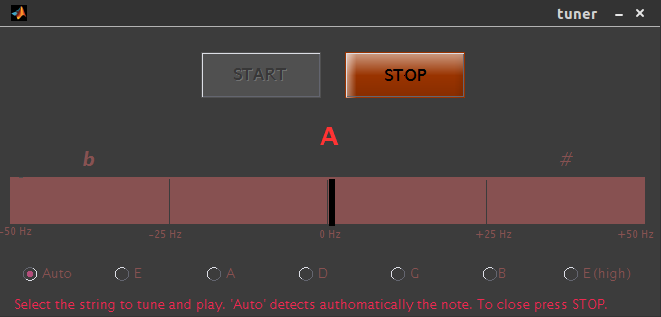
\includegraphics[width=\textwidth*\real{0.8}]{images/ch_08/prestazioni.png}
  \end{center} 
  \caption{\textit{Accordatore in funzione mentre accorda un la con frequenza 110 hz}}  
  \label{fig:accordatore_in_funzione}
\end{figure}

Un altro fattore che può falsare l'operazione di accordatura è la presenza di rumori molto forti vicino al microfono di registrazione. 
In questo caso, infatti, sono presenti delle frequenza aggiuntive che possono essere rilevate dal software.
La soglia introdotta per distinguere il rumore dalla nota, descritta nella sezione \ref{cap:interpolazione}, risulta essere inutile per rumori con frequenze ben determinate. 
Dal momento che rumori di questo tipo risultano essere imprevedibili, si è deciso di non gestirli.
Anche l'accordatore professionale utilizzato come test, infatti, riconosce le frequenza di questa categoria di rumore.
 
La precisione dell'accordatore professionale, di 1 cent, risulta essere maggiore rispetto a quella del software sviluppato, che nel migliore dei casi, grazie all'interpolazione raggiunge valori di 0,5 hz.
La relazione logaritmica che lega cent e frequenza, descritta nella formula \ref{formula:cent} mostra come la precisione raggiunta vari tra i 10 cent, a frequenza 82.4 hz, e i 2.62 cent, a frequenza di 329.6 hz.

\begin{equation}\label{formula:cent}
		\Delta_{f_2-f_1} cent = 1200 \log_2 \left( f_2/f_1 \right)
	\end{equation} 

La divisione in cent riflette la modalità di percezione delle frequenze da parte del sistema uditivo umano, quindi risulta essere una migliore unità di misura per la valutazione della precisione di uno strumento come un accordatore.

Utilizzare una precisione in cent costante, richiede l'utilizzo di una scala logaritmica per l'asse delle frequenze.
Ciò richiedere la sostituzione della trasformata di fourier discreta, che utilizza un numero di campioni costante tra frequenze successive, con altre trasformate.
L'utilizzo di questo tipo di trasformate non è oggetto di questo lavoro.

 

